\section{Experiments}
\label{sec:experiments}

\subsection{Experimental Setup}
\label{sec:exp_setup}

\noindent\textbf{Tasks.}
We use four ordinal benchmarks: Adience~\cite{eidinger2014age} ($K{=}8$ age groups), FairFace~\cite{karkkainen2021fairface} ($K{=}9$ age groups), HCI~\cite{palermo2012dating} ($K{=}5$ decades), and KonIQ-10k~\cite{hosu2020koniq} ($K{=}5$ quality grades from mean-opinion-score quintiles, with cut points fixed on the training split).
Each task is evaluated under six missing-grade patterns: a low, middle, or high grade; two adjacent grades; two separated grades; or both endpoints.
All $K$ grades remain in the test label space.

\noindent\textbf{Adaptation and baselines.}
All main experiments use OpenAI CLIP ViT-B/16~\cite{radford2021clip} with nine adapter configurations covering prompt, ordinal, residual, and cache-based adaptation (details in the supplement), each trained with three seeds, for $9\times4\times6\times3=648$ conditions.
Each run uses 256 training images in total from the seen grades and 64 seen-grade validation images in total.
We compare zero-shot CLIP; the adapted model without and with calibration (Adapted, Adapted+C); two validation-selected global blends with calibration, which choose the blending strength before (Blend-S+C) or jointly with (Blend-A+C) the offset; and TIE+C.
Every calibrated method selects its own largest feasible offset from the registered candidate grid under one common budget: seen-validation nMAE may exceed that of uncalibrated Adapted by at most $\delta=0.005$.
All deployment choices use validation data only; a binary-score control is reported in the supplement.

\noindent\textbf{Metrics.}
MS-AUC averages the pair AUROC of Sec.~\ref{sec:calibration_ranking} over adjacent missing--seen pairs.
Missing MAE averages the per-grade MAE over missing grades; Seen and Overall MAE average over seen and all test images, in grade units.
Results are averaged over masks and seeds within each adapter--dataset setting, then equally over the nine adapters.
Confidence intervals are paired 95\% bootstrap intervals over test groups with fixed checkpoints.

% =========================================================
% TABLE 1 — MAIN RESULTS
% =========================================================

\begin{table*}[t]
\centering
\caption{\textbf{Full-$K$ ordinal grading under matched calibration.}
Means over nine adapter configurations, six missing-grade patterns, and three seeds.
AUC: MS-AUC ($\uparrow$); Miss., Seen, All: MAE over missing-grade, seen-grade, and all test images, in grade units ($\downarrow$).
+C: offset selected on seen-grade validation images under the same budget for every method.
Blend-S/-A: validation-selected global blending, with the strength chosen before or jointly with calibration.
Top block: uncalibrated references.
\textbf{Bold}: best calibrated method.
$\Delta$: TIE+C minus Adapted+C; in MS-AUC, Missing MAE, and Overall MAE, every $\Delta$ has a paired 95\% interval that excludes zero.}
\label{tab:main}
\footnotesize
\setlength{\tabcolsep}{1.5pt}
\begin{tabular*}{\textwidth}{@{\extracolsep{\fill}}l*{16}{c}@{}}
\toprule
& \multicolumn{4}{c}{Adience ($K{=}8$)}
& \multicolumn{4}{c}{HCI ($K{=}5$)}
& \multicolumn{4}{c}{FairFace ($K{=}9$)}
& \multicolumn{4}{c}{KonIQ ($K{=}5$)} \\
\cmidrule(lr){2-5}
\cmidrule(lr){6-9}
\cmidrule(lr){10-13}
\cmidrule(l){14-17}
Method
& AUC & Miss. & Seen & All
& AUC & Miss. & Seen & All
& AUC & Miss. & Seen & All
& AUC & Miss. & Seen & All \\
\midrule
Zero-shot
& 0.880 & 0.816 & 0.747 & 0.738
& 0.621 & 1.193 & 1.108 & 1.134
& 0.806 & 0.789 & 1.055 & 1.095
& 0.547 & 1.218 & 1.200 & 1.207 \\
Adapted
& 0.823 & 1.089 & 0.317 & 0.453
& 0.639 & 1.377 & 0.529 & 0.790
& 0.759 & 1.071 & 0.523 & 0.644
& 0.532 & 1.446 & 0.784 & 0.989 \\
\midrule
Adapted+C
& 0.823 & 0.730 & 0.360 & 0.419
& 0.639 & 1.303 & 0.544 & 0.781
& 0.759 & 0.848 & 0.549 & 0.633
& 0.532 & 1.369 & 0.807 & 0.985 \\
Blend-S+C
& 0.821 & 0.681 & 0.385 & 0.426
& 0.639 & \textbf{1.247} & 0.571 & 0.784
& 0.760 & 0.763 & 0.571 & 0.639
& 0.535 & 1.380 & 0.820 & 0.998 \\
Blend-A+C
& 0.822 & 0.752 & 0.374 & 0.432
& 0.639 & 1.302 & 0.547 & 0.783
& 0.756 & 0.864 & 0.555 & 0.640
& 0.539 & 1.437 & \textbf{0.801} & 1.003 \\
\textbf{TIE+C (ours)}
& \textbf{0.875} & \textbf{0.670}
& \textbf{0.346} & \textbf{0.393}
& \textbf{0.678} & 1.284
& \textbf{0.541} & \textbf{0.772}
& \textbf{0.819} & \textbf{0.749}
& \textbf{0.540} & \textbf{0.617}
& \textbf{0.595} & \textbf{1.348}
& 0.802 & \textbf{0.974} \\
\midrule
$\Delta$
& +0.052 & $-$0.060 & $-$0.015 & $-$0.026
& +0.039 & $-$0.020 & $-$0.004 & $-$0.008
& +0.059 & $-$0.099 & $-$0.010 & $-$0.017
& +0.062 & $-$0.021 & $-$0.005 & $-$0.011 \\
\bottomrule
\end{tabular*}
\end{table*}

\subsection{Main Results under Matched Calibration}
\label{sec:exp_main}

Table~\ref{tab:main} asks the practical question: once every method is calibrated by the same protocol, does ordinal transfer improve full-$K$ grading?
It does.
Relative to Adapted+C, TIE+C raises MS-AUC on all four tasks by 0.039--0.062, and lowers Missing MAE by 0.020--0.099 and Overall MAE by 0.008--0.026.
Seen MAE decreases on every task as well, and the ranking gain holds for 34 of 36 adapter--dataset pairs.
Adapted and Adapted+C have identical MS-AUC, as Proposition~\ref{prop:cal} predicts: calibration moves decisions, not the order.

Global blending is a strong baseline in principle, but not in deployment.
Validation-selected Blend stays within 0.007 MS-AUC of Adapted on every task.
Seen-only validation selects for seen-grade performance and does not directly optimize missing--seen ranking.
TIE+C therefore achieves higher MS-AUC and lower Overall MAE than both Blend variants on all four tasks, and lower Missing MAE than Blend-A+C on all four.
Blend-S+C reaches a lower Missing MAE on HCI (1.247 vs.\ 1.284), at the cost of higher Overall MAE.
Section~\ref{sec:exp_matched} asks whether any blending strength, even one chosen with test labels, could close the gap.

\subsection{Ordinal Transfer beyond Global Blending}
\label{sec:exp_matched}

Because TIE is linear, it commutes with blending (Proposition~\ref{prop:tie_structure}), so the two can be compared at matched strength in a controlled intervention: at every $\lambda$ they share all seen-grade scores and differ only in where the missing grade's displacement comes from (Fig.~\ref{fig:matched_strength}).
This analysis uses the three interior patterns (81 conditions per dataset) and measures ranking only.
Under pointwise paired intervals, TIE improves missing--seen ranking at all 16 nonzero strengths on FairFace and KonIQ and at 14 and 13 of 16 on Adience and HCI; the only negative interval is HCI at $\lambda=0.1$.
At $\lambda=1$, TIE gains 0.038--0.069 MS-AUC, with positive point estimates in 35 of 36 interior adapter--dataset settings.
More importantly, tuning the strength does not close the gap.
By Proposition~\ref{prop:family}, calibrated blending moves along a single path of rankings; let the best Blend be the maximum of its adapter-averaged curve over the 17 evaluated strengths---a single $\lambda$ shared by all configurations and selected retrospectively on the test results.
On HCI, FairFace, and KonIQ, TIE at $\lambda=1$ still exceeds it by 0.042, 0.018, and 0.067, and exceeds the zero-shot reference by 0.113, 0.025, and 0.096: the gain is transfer, not a return to zero-shot.
Adience shows the complementary regime: zero-shot already ranks age well, the best Blend ($\lambda=0.1$) stays slightly above TIE at $\lambda=1$, and TIE instead recovers 79\% of the ranking lost to adaptation and degrades three times more slowly with $\lambda$.
The key is not merely how much adaptation is retained, but where the missing grade's displacement comes from.

% =========================================================
% FIGURE 2 — EXISTING FROZEN ARTIFACT
% =========================================================

\begin{figure*}[t]
\centering
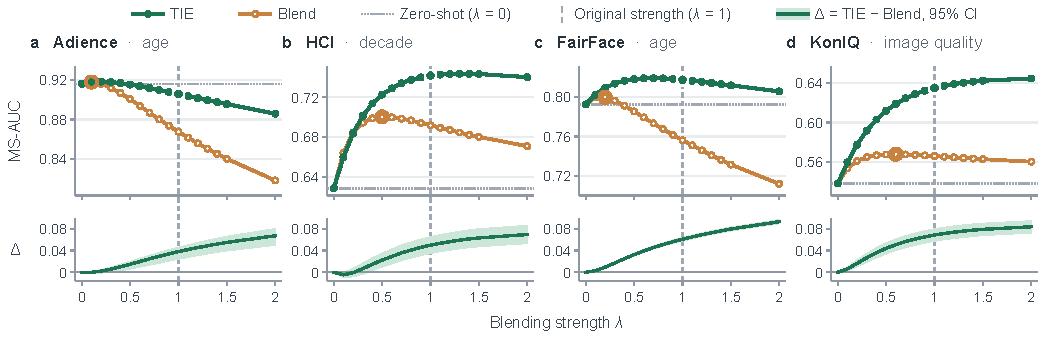
\includegraphics[width=\textwidth]{figures/fig2.pdf}
\caption{\textbf{Ordinal transfer beyond global blending.} Top: MS-AUC under interior missing-grade masks for global score blending $T+\lambda D$ (Blend) and for TIE at the same strength, $T+\lambda\mathcal{L}_{\mathcal{U}}(D)$, equally averaged over nine adapter configurations (81 conditions per dataset: 9 configurations $\times$ 3 masks $\times$ 3 seeds). At every $\lambda$ the two share all seen-grade scores and differ only in the missing grades' displacement. The curves meet at the zero-shot reference ($\lambda=0$); $\lambda=1$ is the original adaptation strength, and $\lambda>1$ extrapolates. Enlarged markers: the best Blend on the 17-point grid and TIE at $\lambda=1$. Bottom: paired difference $\Delta$ = TIE $-$ Blend with pointwise 95\% bootstrap intervals. Upper panels share the same vertical span.}
\label{fig:fig2}
\label{fig:matched_strength}
\end{figure*}

\subsection{When and Why Transfer Helps}
\label{sec:exp_structure}

\noindent\textbf{Endpoints versus interior grades.}
The endpoint guarantee of Proposition~\ref{prop:tie_structure} is not vacuous: on endpoint patterns, adaptation lowers MS-AUC below zero-shot on all four tasks, by 0.065, 0.028, 0.058, and 0.056 on Adience, HCI, FairFace, and KonIQ, and TIE restores the zero-shot ranking exactly.
On interior patterns TIE goes further and exceeds zero-shot on three tasks (Sec.~\ref{sec:exp_matched}), so neighbors contribute task information that the zero-shot model lacks.

\noindent\textbf{Grade-specific supervision.}
Transfer helps most where it is needed most.
In two support studies, one fixing the total training budget and the other fixing the seen-grade images, the average ranking gain of TIE decreases monotonically as missing-grade support grows from 0\% to 10\% to 20\%, in all 18 method--task--protocol summaries.
Inheritance is most valuable exactly when a grade has no images of its own.

\noindent\textbf{How much: a full-support reference.}
Table~\ref{tab:controls}a compares TIE with FullSup, a budget-matched model adapted on all grades.
Without a single image of the missing grade, TIE closes 44--58\% of the Missing-MAE gap on three tasks and more than the whole gap on KonIQ, where it beats FullSup for eight of nine adapters.
FullSup is an empirical reference rather than an upper bound, because it spreads the same budget over more grades.

\noindent\textbf{Knowledge preservation is not order preservation.}
KgCoOp~\cite{yao2023kgcoop} keeps learned prompts close to zero-shot knowledge.
On HCI, it improves Missing MAE over CoOp by 0.074 yet lowers MS-AUC by 0.118 (Table~\ref{tab:controls}b): it fixes the score at the expense of the order.
TIE on top of KgCoOp raises MS-AUC on all four tasks, by 0.030--0.157, although its calibrated Missing MAE is higher than KgCoOp's on three of them.
The supplement compares TIE with direct score interpolation and with distance-weighted and one-sided variants, and splits the inheritance error of Proposition~\ref{prop:tie_error} into its constant and image-dependent parts.

% =========================================================
% TABLE 2 — SINGLE-COLUMN CONTROLS
% =========================================================

\begin{table}[t]
\centering
\caption{\textbf{Supervision and training-time controls.}
(a) Uncalibrated Missing MAE of Adapted, TIE, and a budget-matched full-support model (FullSup); Closed: share of the Adapted--FullSup gap closed by TIE, averaged over the nine adapters.
(b) KgCoOp-style adaptation on two interior patterns: change from CoOp, and the MS-AUC gain of TIE applied on top of KgCoOp.}
\label{tab:controls}
\small
\setlength{\tabcolsep}{4pt}
\textit{(a) Full-support reference}\par\vspace{2pt}
\begin{tabular}{@{}lcccc@{}}
\toprule
Dataset & Adapted$\downarrow$ & TIE$\downarrow$ & FullSup$\downarrow$ & Closed \\
\midrule
Adience & 1.089 & 0.685 & 0.418 & 58\% \\
HCI & 1.377 & 1.052 & 0.642 & 44\% \\
FairFace & 1.071 & 0.696 & 0.417 & 56\% \\
KonIQ & 1.446 & 0.883 & 0.938 & 111\% \\
\bottomrule
\end{tabular}
\par\vspace{6pt}
\textit{(b) KgCoOp: knowledge preservation vs.\ order}\par\vspace{2pt}
\begin{tabular}{@{}lccc@{}}
\toprule
& \multicolumn{2}{c}{KgCoOp $-$ CoOp} & TIE on KgCoOp \\
\cmidrule(lr){2-3}\cmidrule(l){4-4}
Dataset & $\Delta$MS-AUC & $\Delta$Miss.\ MAE & $\Delta$MS-AUC \\
\midrule
Adience & $+$0.011 & $+$0.045 & $+$0.030 \\
HCI & $-$0.118 & $-$0.074 & $+$0.157 \\
FairFace & $-$0.004 & $-$0.001 & $+$0.045 \\
KonIQ & $-$0.005 & $-$0.013 & $+$0.055 \\
\bottomrule
\end{tabular}
\end{table}

\subsection{Generality}
\label{sec:exp_generality}

Table~\ref{tab:extensions} varies one factor at a time, each within its own protocol.
TIE raises MS-AUC with LAION-pretrained weights~\cite{cherti2023reproducible} on Adience and HCI, with a ResNet-50 backbone on HCI, and on a new task, facial-beauty grading on SCUT-FBP5500~\cite{liang2018scut}, for both CoOp and OrdinalCLIP-style adaptation (by 0.120 and 0.188).
With full fine-tuning of the visual encoder, it raises MS-AUC on HCI, FairFace, and KonIQ by 0.008, 0.010, and 0.199, and leaves Adience essentially unchanged ($-0.006$).
On diabetic-retinopathy grading (DDR~\cite{li2019ddr}), TIE lowers Missing MAE under all three backbones tested, but its ranking effect is mixed across backbones (supplement).

% =========================================================
% TABLE 3 — SINGLE-COLUMN EXTENSIONS
% =========================================================

\begin{table}[t]
\centering
\caption{\textbf{Generality.} TIE minus Adapted, both uncalibrated, within each extension protocol (not pooled with Table~\ref{tab:main}). $\Delta$AUC: MS-AUC; $\Delta$Miss.: Missing MAE. SCUT-FBP5500 uses its five official folds.}
\label{tab:extensions}
\footnotesize
\setlength{\tabcolsep}{3pt}
\begin{tabular}{@{}lllcc@{}}
\toprule
Factor & Setting & Adapter & $\Delta$AUC$\uparrow$ & $\Delta$Miss.$\downarrow$ \\
\midrule
Pretrain. & LAION, Adience & CoOp & $+$0.032 & $-$0.511 \\
& LAION, HCI & CoOp & $+$0.043 & $-$0.189 \\
Backbone & RN50, HCI & CoOp & $+$0.071 & $-$0.237 \\
Domain & SCUT-FBP5500 & CoOp & $+$0.120 & $-$0.059 \\
& SCUT-FBP5500 & OrdinalCLIP & $+$0.188 & $-$0.083 \\
\bottomrule
\end{tabular}
\end{table}
